%%%%%%%%%%%%%%%%%%%%% {{{
%%Options for presentations (in-class) and handouts (e.g. print).
\documentclass[pdf,9pt]{beamer}


%%%%%%%%%%%%%%%%%%%%%%
%Change this for different slides so it appears in bar
\usepackage{authoraftertitle}
\date{\S AppendixA. Complex Numbers}

%%%%%%%%%%%%%%%%%%%%%%
%% Upload common style file
\usepackage{LyryxLAWASlidesStyle}

\begin{document}

%%%%%%%%%%%%%%%%%%%%%%%
%% Title Page and Copyright Common to All Slides

%Title Page
\input frontmatter/titlepage.tex

%LOTS Page
\input frontmatter/lyryxopentexts.tex

%Copyright Page
\input frontmatter/copyright.tex

%%%%%%%%%%%%%%%%%%%%%%%%% }}}

%-------------- start slide -------------------------------%{{{ 2
\begin{frame}[fragile]
   \tableofcontents
\end{frame}
%-------------- end slide -------------------------------%}}}

\section[\textcolor{yellow}{}]{\textcolor{yellow}{Complex Numbers}}

%-------------- start slide -------------------------------%{{{ 3
\frame{
\frametitle{Complex Numbers}
\pause
\begin{block}{ Why complex numbers?}
  \begin{itemize}
    \item Counting numbers: $1, 2, 3, 4, 5, \ldots$
    \item<2-> Integers: $0, 1, 2, 3, 4 \ldots$ but also
      $-1, -2, -3 \ldots$
    \item<3->
      To solve $3x+2=0$, integers aren't enough,
      so we have \alert{rational numbers} (fractions), i.e.,
      \[ \mbox{if } 3x+2 = 0, \mbox{ then } x=-\frac{2}{3}.\]
    \item<4->
      We still can't solve $x^2-2=0$ because there are no rational
      numbers $x$ with the property that $x^2-2=0$, so we have
      \alert{irrational numbers}, i.e.,
      \[ \mbox{if } x^2-2 = 0, \mbox{ then } x=\pm\sqrt{2}.\]
    \item<5->
      The set of \alert{real numbers}, $\RR$, consists of all
      rational and irrational numbers (note that integers are
      rational numbers).  However, we still can't solve
      \[ x^2+1 = 0\]
      because this requires $x^2=-1$, but any \alert{real} number
      $x$ has the property that $x^2\geq 0$.
  \end{itemize}
\end{block}
}
%-------------- end slide -------------------------------%}}}

%-------------- start slide  -------------------------------%{{{ 4
\frame{
\begin{definitions}
  \begin{itemize}
    \item The \alert{imaginary unit}, denoted $i$, is defined to be a number with the property that $i^2=-1$. \pause
    \item A \alert{pure imaginary} number has the form $bi$ where $b\in\RR$, $b\neq 0$, and $i$ is the imaginary unit. \pause
    \item A \alert{complex number} is any number $z$ of the form
      \[ z = a + bi\]
      where $a,b\in\RR$ and $i$ is the imaginary unit. \\[1em] \pause
      (1) $a$ is called the \alert{real part} of $z$. \\[1em] \pause
      (2) $b$ is called the \alert{imaginary part} of $z$ \\[1em] \pause
      (3) If $b=0$, then $z$ is a real number.
  \end{itemize}
\end{definitions}
}
%-------------- end slide -------------------------------%}}}

%-------------- start slide -------------------------------%{{{  5
\frame{
\begin{block}{The Complex Plane}
    \pause
    A complex number $z=a+bi$ can be represented geometrically
    by the point $(a,b)$ in the $xy$-plane, where
    the $x$-axis is the \alert{real axis} and the $y$-axis is
    the \alert{imaginary axis}.

    \pause
	\begin{picture}(3,2.1)
	\put(1,0){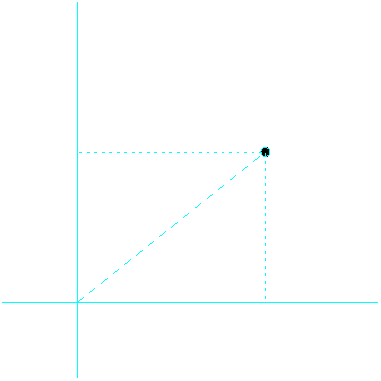
\includegraphics[scale=.8]{figures/complex-plane_neg.pdf}}
	{\small
	\put(1.25,0.2){$0$}
	\put(2.8,0.2){$x$}
	\put(1.23,1.6){$y$}
	\put(2.5,1.2){$(a,b)$}}
	{\footnotesize
	\put(1.9,1.25){$a$}}
	\put(2.45,0.8){$b$}
    \end{picture}
    \pause
    \begin{itemize}
	\item Real numbers: $a+0i$ lie on the $x$-axis.  \pause
	\item Pure imaginary numbers: $0 + bi$ ($b\neq 0$) lie on the $y$-axis.
    \end{itemize}
\end{block}
}
%-------------- end slide -------------------------------%}}}

%-------------- start slide  -------------------------------%{{{ 6
\frame{
\begin{block}{Addition and Subtraction of Complex Numbers}
  \pause
  Let $\textcolor{blue}{z=a+bi}$ and
  $\textcolor{orange}{w=c+di}$ be complex numbers.
  \pause
  \begin{itemize}
  \item
  \alert{Equality}
  $\textcolor{blue}{z}=\textcolor{orange}{w}$ if and
  $\textcolor{blue}{a}=\textcolor{orange}{c}$ and
  $\textcolor{blue}{b}=\textcolor{orange}{d}$.
  \pause
  \item
  \alert{Addition}
  \vspace*{-.1in}
  \pause

  \[ \textcolor{blue}{z} + \textcolor{orange}{w}
  = \pause \textcolor{blue}{(a+bi)} + \textcolor{orange}{(c+di)}
  = \pause  (\textcolor{blue}{a}+\textcolor{orange}{c})
  + (\textcolor{blue}{b}+\textcolor{orange}{d})i. \]
  \vspace*{-.1in}

  \pause
  \item
  \alert{Subtraction}
  \vspace*{-.1in}
  \pause

  \[ \textcolor{blue}{z} - \textcolor{orange}{w}
  = \textcolor{blue}{(a+bi)} - \textcolor{orange}{(c+di)}
  =  (\textcolor{blue}{a}-\textcolor{orange}{c})
  + (\textcolor{blue}{b}-\textcolor{orange}{d})i. \]
  \end{itemize}
\end{block}
\pause
\vfill
\begin{examples}
  \begin{itemize}
    \item $(-3+6i) + (5-i) = \pause 2+5i$.
    \pause
    \item $(4-7i) + (6-2i) = \pause 10-9i$.
    \pause
    \item $(-3+6i) - (5-i) = \pause -8+7i$.
    \pause
    \item $(4-7i) - (6-2i) = \pause -2-5i$.
  \end{itemize}
\end{examples}
}
%-------------- end slide -------------------------------%}}}

%-------------- start slide  -------------------------------%{{{ 7
\frame{
\begin{block}{Properties of Addition}
  \pause
  Let $z$, $w$, and $v$ be complex numbers.
  \pause
  \begin{enumerate}
  \item $z + w = w + z$.
  \hfill{\textcolor{blue}{(addition is commutative)}}
  \medskip
  \pause
  \item $(z + w) + v = z + (w + v)$.
  \hfill{\textcolor{blue}{(addition is associative)}}
  \medskip
  \pause
  \item $z + 0 = z$.
  \hfill{\textcolor{blue}{(existence of an additive identity)}}
  \medskip
  \pause
  \item
  For every $z=a+bi$ there exists a complex number $-z = -a -bi$ such that
  $z + (-z) = 0$.
  \hfill{\textcolor{blue}{(existence of an additive inverse)}}
  \end{enumerate}
\end{block}
}
%-------------- end slide -------------------------------%}}}

%-------------- start slide  -------------------------------%{{{ 8
\frame{
\begin{block}{Addition in the Complex Plane}
  \pause
  If $z=a+bi$ and $w=c+di$, then $z+w=(a+c)+(b+d)i$.
  \pause
  Geometrically, we have:
  \bigskip

  \begin{picture}(3,2)
  \put(1.25,0){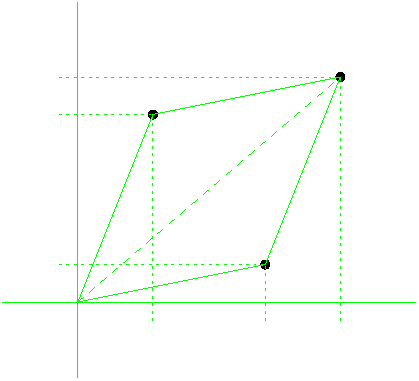
\includegraphics[scale=.75]{figures/addition_neg.pdf}}
  {\small
  \put(1.5,0.25){$0$}
  \put(3.2,0.25){$x$}
  \put(1.5,1.75){$y$}
  \put(2.65,0.54){$z$}
  \put(1.93,1.40){$w$}
  \put(3.00,1.50){$z+w$}
  }
  {\footnotesize
  \put(1.98,0.20){$c$}
  \put(2.53,0.20){$a$}
  \put(2.81,0.20){$a+c$}
  \put(1.45,0.55){$b$}
  \put(1.45,1.30){$d$}
  \put(1.22,1.48){$b+d$}
  }
  \end{picture}
  \bigskip
  \pause

  $0$, $z$, $w$, and $z+w$ are the vertices of a parallelogram.
\end{block}
}
%-------------- end slide -------------------------------%}}}

%-------------- start slide  -------------------------------%{{{ 9
\frame{
\begin{block}{Multiplication of Complex Numbers}
  Let $z=a+bi$ and $w=c+di$ be complex numbers.
  Then the \alert{product} of $z$ and $w$ is
  \[ zw=(a+bi)(c+di) = (ac-bd)+(ad+bc)i.\]
  \pause
  \alert{The multiplication is done essentially as the product of
  two linear polynomials, with $i^2$ replaced by $-1$.}
\end{block}
\vfill
\pause
\begin{example}
  \vspace{-1em}
  \begin{eqnarray*}
    (2-3i)(-3+4i) = & = & ((2)(-3) - (-3)(4))+((2)(4)+(-3)(-3))i \\
                    & = & (-6 + 12) + (8 + 9)i                   \\
                    & = & 6+17i
  \end{eqnarray*}
\end{example}
}
%-------------- end slide -------------------------------%}}}

%-------------- start slide  -------------------------------%{{{ 10
\frame{
\begin{block}{Properties of Multiplication}
\pause
Let $z, w$ and $v$ be complex numbers.
\pause
\begin{itemize}
\item $zw=wz$.
\hfill{\textcolor{blue}{(multiplication is commutative)}}
\medskip
\pause
\item $(zw)v=z(wv)$.
\hfill{\textcolor{blue}{(multiplication is associative)}}
\medskip
\pause
\item $z (w+v) = zw + zv$.
\hfill{\textcolor{blue}{(multiplication distributes over addition)}}
\medskip
\pause
\item $1z=z$.
\hfill{\textcolor{blue}{(`1' is the multiplicative identity)}}
\medskip
\pause
\item
For each $z \neq 0$, there exists $z^{-1}$ such that
$z z^{-1} = 1$.\\
\hfill{\textcolor{blue}{(existence of a multiplicative inverse)}}
\end{itemize}
\end{block}
}
%-------------- end slide -------------------------------%}}}

%-------------- start slide -------------------------------%{{{ 11
\frame{
\begin{problem}
Find all complex numbers $z$ so that $z^2=-3+4i$.
\end{problem}
\pause
\begin{solution}
Let $z=a+bi$.  Then
\vspace*{-.15in}

\[ z^2=(a+bi)^2=(a^2-b^2)+2abi = -3+4i,\]
\vspace*{-.3in}

\pause
so
\[ a^2-b^2=-3 \quad\text{and}\quad 2ab=4.\]
\vspace*{-.25in}

\pause
Since $2ab=4$, $a=\frac{2}{b}$.
\pause
Substituting this into
the first equation gives us
\pause
\begin{eqnarray*}
a^2-b^2 & = & -3 \\
\left(\frac{2}{b}\right)^2 - b^2 & = & -3 \\ \pause
\frac{4}{b^2} - b^2 & = & -3 \\ \pause
4- b^4 & = & -3b^2 \\ \pause
b^4-3b^2-4 & = & 0.
\end{eqnarray*}

\vspace*{-.1in}
\end{solution}
}
%-------------- end slide -------------------------------%}}}

%-------------- start slide -------------------------------%{{{ 12
\frame{
\begin{solution}[continued]
Now, $b^4-3b^2-4=0$ can be factored \pause into
\begin{eqnarray*}
(b^2-4)(b^2+1)& = & 0\\
\pause
(b-2)(b+2)(b^2+1)& = & 0.
\end{eqnarray*}
\pause
Since $b\in \RR$ and $b^2+1$ has no real roots, $b=2$ or $b=-2$.
\bigskip
\pause

Since $a=\frac{2}{b}$, it follows that
\pause
\begin{itemize}
\item when $b=2$, $a=1$, and $z=a+bi=1+2i$;
\pause
\item when $b=-2$, $a=-1$, and $z=a+bi=-1-2i$.
\pause
\end{itemize}

\bigskip
Therefore, if $z^2=-3+4i$, then $z=1+2i$ or $z=-1-2i$.
\end{solution}
}
%-------------- end slide -------------------------------%}}}

%-------------- start slide -------------------------------%{{{ 13
\frame{
\begin{block}{The Conjugate of a Complex Number}
    \pause
    Let $z=a+bi$ be a complex number.
    \pause
    The \alert{conjugate} of $z$ is the complex number
    \alert{$\overline{z}=a-bi$}.
    \pause
    Geometrically, $\overline{z}$ is the reflection of $z$ in the $x$-axis.
    \pause

    \begin{picture}(3,1.27)
    \put(1.2,0){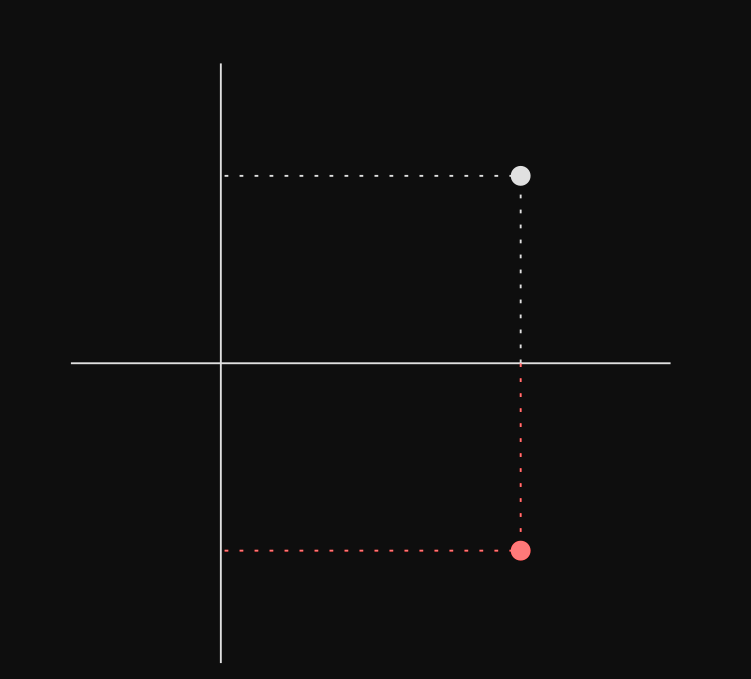
\includegraphics[scale=.14]{figures/conjugate.png}}
    {\footnotesize
    \put(1.4,0.5){$0$}
    \put(1.4,1.1){$y$}
    \put(2.3,0.5){$x$}
    \put(2.2,1.0){$(a,b)$}
    \put(2.2,0.2){\alert{$(a,-b)$}}
    }\end{picture}
\end{block}
\vfill
\pause
\begin{examples}
    \begin{itemize}
        \pause
        \item If $z=3+4i$, then $\overline{z}=\pause 3-4i$,
            \pause
            i.e., $\overline{3+4i}=3-4i$.
            \pause
            \medskip

        \item $\overline{-2+5i}=\pause -2-5i$.
            \pause
            \medskip

        \item $\overline{i}=\pause -i$.
            \pause
            \medskip

        \item $\overline{7}=\pause 7$.
    \end{itemize}
\end{examples}
}
%-------------- end slide -------------------------------%}}}

%-------------- start slide -------------------------------%{{{ 14
\frame{
\begin{block}{Properties of the Conjugate}
    Let $z$ and $w$ be complex numbers.
    \begin{itemize}
        \item $\overline{z\pm w} = \overline{z} \pm \overline{w}$.
            \pause
            \item
            $\overline{(zw)} = \overline{z}~ \overline{w}$.
            \medskip
            \pause
        \item $\overline{(\overline{z})}=z$.
            \pause
            \medskip
        \item $\overline{\left(\frac{z}{w}\right)} =
            \frac{\overline{z}}{\overline{w}}$.
            \pause
            \medskip
        \item $z$ is real if and only if $\overline{z}=z$.
    \end{itemize}
\end{block}
\pause
\begin{remark}
    If $z=a+bi$, then
    \pause
    \[ z\overline{z}= \pause (a+bi)(a-bi)= \pause a^2 + b^2.\]
\end{remark}
}
%-------------- end slide -------------------------------%}}}

%-------------- start slide -------------------------------%{{{ 15
\frame{
\begin{block}{Division of Complex Numbers}
    \pause
    Let $z=a+bi$ and $w=c+di$ be complex numbers.
    \pause
    Suppose that $c,d$ are not both zero.
    \pause
    Then the \alert{quotient $z$ divided by $w$} is
    \begin{eqnarray*}
    \frac{z}{w}= \pause \frac{a+bi}{c+di} & = & \pause\frac{a+bi}{c+di}\times \frac{c-di}{c-di} \\
                                          & = & \pause\frac{(ac+bd)+(bc-ad)i}{c^2+d^2}          \\
                                          & = & \pause\frac{ac+bd}{c^2+d^2} +\frac{bc-ad}{c^2+d^2}i.
    \end{eqnarray*}
    \pause
    \alert{The quotient $\frac{z}{w}$ is obtained by multiplying
    both top and bottom of $\frac{z}{w}$ by $\overline{w}$ and
    then simplifying the expression.}
\end{block}
}
%-------------- end slide -------------------------------%}}}

%-------------- start slide -------------------------------%{{{ 16
\frame{
\begin{examples}
    \pause
    \begin{itemize}
        \item
        \[ \frac{1}{i} = \pause \frac{1}{i}\times \frac{-i}{-i}
                       = \frac{-i}{-i^2}
                       = -i. \]
        \pause
        \item
        {\small
        \[ \frac{2-i}{3+4i} = \pause \frac{2-i}{3+4i}\times \frac{3-4i}{3-4i}
                            = \frac{(6-4)+(-3-8)i}{3^2+4^2}
                            = \frac{2-11i}{25}
                            = \frac{2}{25} - \frac{11}{25}i. \]}
        \pause
        \item
        {\small
        \[ \frac{1-2i}{-2+5i} = \pause \frac{1-2i}{-2+5i}\times \frac{-2-5i}{-2-5i}
                              = \frac{(-2-10) + (4-5)i}{2^2+5^2}
                              = -\frac{12}{29}-\frac{1}{29}i.  \]}
    \end{itemize}
\end{examples}
}
%-------------- end slide -------------------------------%}}}

%-------------- start slide -------------------------------%{{{ 17
\frame{
\begin{block}{The Multiplicative Inverse}
    Every nonzero complex number $z=a+bi$ has a unique
    \alert{multiplicative inverse} $z^{-1}=\frac{1}{z}$ such that
    $zz^{-1} = 1$, and
    \pause
    \[ \frac{1}{z} =
    \pause
    \frac{1}{z}\times \frac{\overline{z}}{\overline{z}} =
    \pause
    \frac{\overline{z}}{z\overline{z}} =
    \pause
    \frac{a-bi}{a^2+b^2} =
    \pause
    \frac{a}{a^2+b^2}-\frac{b}{a^2+b^2}i.\]
    \pause
    \alert{Since $z$ is nonzero, $a^{2} + b^{2} \neq 0$, so the inverse is defined.}
\end{block}
\pause
\vfill
\begin{example}
    When $z = 2 + 6i$, $z^{-1}$ is defined, and
    \pause
    \[ \frac{1}{z}=
    \frac{1}{2+6i} =
    \pause
    \frac{1}{2+6i}\times \frac{2-6i}{2-6i}=
    \pause
    \frac{2-6i}{2^2+6^2} =
    \pause
    \frac{2-6i}{40} =
    \pause
    \frac{1}{20} -  \frac{3}{20}i. \]
    \pause
    \alert{You can always check that $zz^{-1}=1$.}
\end{example}
}
%-------------- end slide -------------------------------%}}}

\section[\textcolor{yellow}{}]{\textcolor{yellow}{Modulus}}

%-------------- start slide -------------------------------%{{{ 18
\frame{
\frametitle{Modulus}
\pause
\begin{definition}
    The \alert{absolute value} or \alert{modulus} of a complex
    number $z=a+bi$ is
    \[ \left| z \right| = \sqrt{a^2+b^2}\]
    \pause
    {\em Note that this is consistent with the definition of the
    absolute value of a real number.}
    \medskip
    \pause

    Geometrically,  $|z|=\sqrt{a^2+b^2}$ is the distance from $z$ to the origin.

    \begin{picture}(3,1.1)
    \put(1.2,0){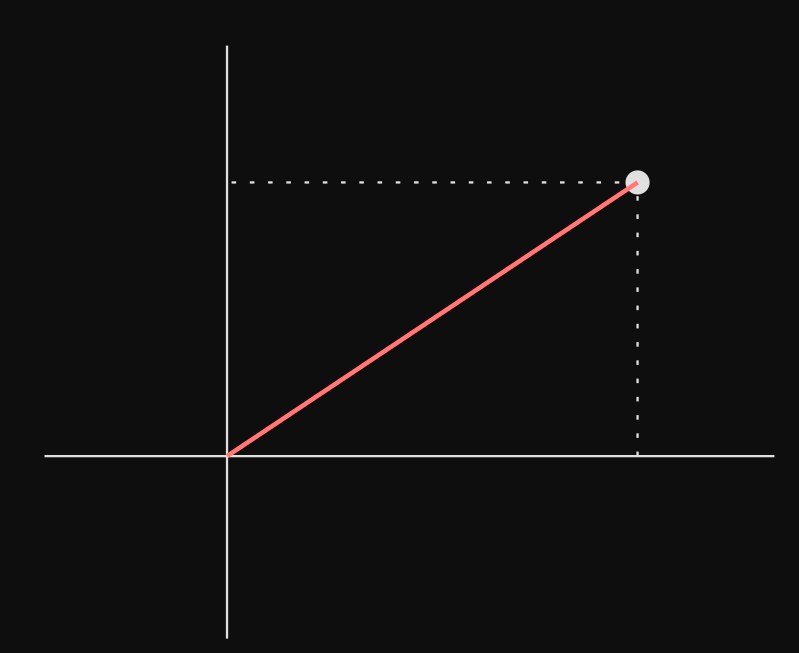
\includegraphics[scale=.115]{figures/absolute-value.png}}
    {\footnotesize
    \put(1.4,0.2){$0$}
    \put(1.4,0.9){$y$}
    \put(2.3,0.2){$x$}
    \put(2.25,0.8){$(a,b)$}}
    {\scriptsize
    \put(1.8,0.2){$a$}
    \put(2.25,0.5){$b$}}
    {\tiny
    \put(1.55,0.62){\alert{$\sqrt{a^2+b^2}$}}
    }\end{picture}
\end{definition}
}
%-------------- end slide -------------------------------%}}}

%-------------- start slide -------------------------------%{{{ 19
\frame{
\begin{examples}
    \pause
    \begin{enumerate}
        \item $|-3+4i|=
            \pause
            \sqrt{3^2+4^2}=
            \pause \sqrt{25}=\pause 5$.
            \pause

            \medskip
        \item $|3-2i|=\pause \sqrt{3^2+2^2}=\sqrt{13}$.
            \pause

            \medskip
        \item $|i|=\pause \sqrt{1^2}=1$.
    \end{enumerate}
\end{examples}
}
%-------------- end slide -------------------------------%}}}

%-------------- start slide -------------------------------%{{{ 20
\frame{

\begin{theorem}[ Properties of the Modulus ]
    \pause
    Let $z$ and $w$ be complex numbers.
    \pause
    \begin{enumerate}
        \item
        $z \cdot \overline{z} = |z|^2$.
        \pause
        \item
        $\frac{1}{z}= \frac{\overline{z}}{|z|^2}$.
        \pause
        \item
        $|z|\geq 0$ for all $z$.
        \pause
        \item
        $|z|=0$ if and only if $z=0$.
        \pause
        \item
        $|zw|=|z|~|w|$.
        \pause
        \item
        $\left|\frac{z}{w}\right| =\frac{|z|}{|w|}$.
        \pause
        \item \textcolor{blue}{The Triangle Inequality}

        $|z+w|\leq |z|+|w|$.
    \end{enumerate}
\end{theorem}
}
%-------------- end slide -------------------------------%}}}

%-------------- start slide -------------------------------%{{{ 21
\frame{
\begin{example}[ The Triangle Inequality: Geometrically ]
    If $z=a+bi$ and $w=c+di$, then $|z-w|=\sqrt{(a-c)^2+(b-d)^2}$.
    \pause

    \begin{picture}(3,1.4)
    \put(1.25,0){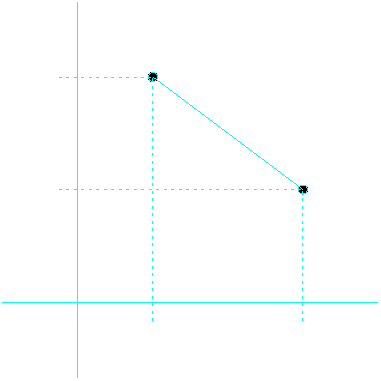
\includegraphics[scale=.5]{figures/difference_neg.pdf}}
    {\small
    \put(1.35,0.1){$0$}
    \put(2.4,0.1){$x$}
    \put(1.35,1.15){$y$}
    \put(1.85,1.05){$z=a+bi$}
    \put(2.35,0.6){$w=c+di$}}
    {\tiny
    \put(1.35,1.0){$b$}
    \put(1.35,0.6){$d$}
    \put(1.51,0.8){$b-d$}
    \put(1.9,0.55){$c-a$}
    \put(1.73,0.1){$a$}
    \put(2.23,0.1){$c$} }
    \end{picture}
    \bigskip

    This shows that the \alert{distance} between
    $z$ and $w$ in the complex plane is just the absolute value
    of their difference.
\end{example}
}
%-------------- end slide -------------------------------%}}}

%-------------- start slide -------------------------------%{{{ 22
\frame{
\begin{example}[continued]
    Now consider the points $z$, $z+w$, and the origin $0$
    in the complex plane.
    \pause

    \begin{picture}(3,2)
    \put(1.25,0){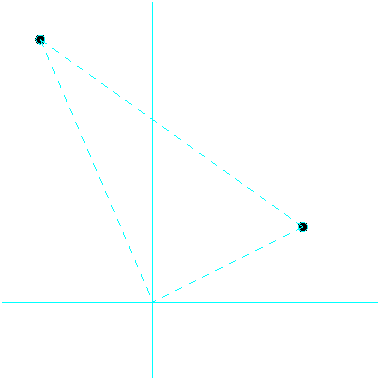
\includegraphics[scale=.75]{figures/triangle-ineq_neg.pdf}}
    {\small
    \put(1.9,0.25){$0$}
    \put(3.0,0.25){$x$}
    \put(2.05,1.75){$y$}
    \put(1.28,1.78){$z+w$}
    \put(2.85,0.73){$z$}}
    {\tiny
    \put(1.40,0.95){$|z+w|$}
    \put(2.10,1.27){$|w|$}
    \put(2.25,0.62){$|z|$}
    }
    \end{picture}
    \pause

    The triangle formed by these points has sides of length $|z|$,
    and $|z+w|$ and $|w|$ (the absolute value of the difference
    between $z+w$ and $z$).
    \pause

    Since the length of \alert{any} side of a triangle is at most the
    sum of the lengths of the other two sides, we get
    \alert{$|z+w|\leq |z|+|w|$.}
\end{example}
}
%-------------- end slide -------------------------------%}}}

\section[\textcolor{yellow}{}]{\textcolor{yellow}{Complex Numbers in Polar Form}}

%-------------- start slide -------------------------------%{{{ 23
\frame{
\frametitle{Complex Numbers in Polar Form}
\pause
\begin{emptytitle}
    Suppose $z=a+bi$, and let $\textcolor{blue}{r}=|z|=\sqrt{a^2+b^2}$.
    Then $\textcolor{blue}{r}$ is the distance from $z$ to the origin.
    Denote by $\alert{\theta}$ the angle that the line through $0$ and $z$
    makes with the positive $x$-axis (measured clockwise).

    \begin{picture}(3,1.75)
    \put(1.25,0){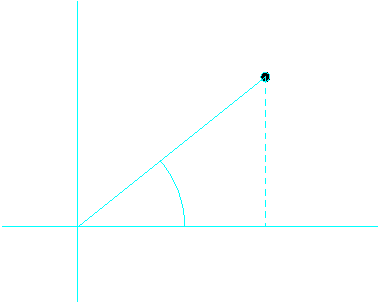
\includegraphics[scale=.75]{figures/polar_neg.pdf}}
    {\small
    \put(1.5,0.25){$0$}
    \put(2.9,0.25){$x$}
    \put(1.5,1.3){$y$}
    \put(2.65,1.1){$z=a+bi$}
    \put(2.15,0.25){$a$}
    \put(2.6,0.7){$b$}
    \put(2.05,0.8){$\textcolor{blue}{r}$}
    \put(1.85,0.43){$\alert{\theta}$}
    }
    \end{picture}

    \pause
    Then $\theta$ is an angle defined by
    $\cos\theta = \frac{a}{r}$ and $\sin\theta=\frac{b}{r}$, so

    \vspace*{-.15in}
    \[ z=r\cos\theta +r\sin\theta i=r(\cos\theta + i\sin\theta).\]

    \pause
    $\theta$ is called \alert{an argument of $z$}, and is
    denoted $\arg z$.
\end{emptytitle}
}
%-------------- end slide -------------------------------%}}}

%-------------- start slide -------------------------------%{{{ 24
\frame{
\begin{definition}[Polar Form of a Complex Number]
    Let $z$ be  a complex number with $|z|=r$ and $\arg z=\theta$.
    Then
    \[ z=re^{i\theta}=r(\cos\theta + i\sin\theta )\]
    is called \alert{a polar form} of $z$.
\end{definition}
\vfill
\pause
\begin{remark}
    Since $\arg z$ is not unique, we do not write \alert{the}
    polar form of $z$.
\end{remark}
\vfill
\pause
\begin{definition}
    Let $z$ be a complex number with $|z|=r$.
    The \alert{principal argument} of $z$
    is the unique angle $\theta=\arg z$ (measured in radians) such that
    \[ -\pi < \theta \leq \pi. \]
\end{definition}
}
%-------------- end slide -------------------------------%}}}

%-------------- start slide -------------------------------%{{{ 25
\frame{
\begin{example}
    Find the polar form for the number $z=1$.
\end{example}
\pause
\vfill
\begin{solution}
    To convert $z$ to polar form, we need to find $r$ and $\theta$
    so that $1=re^{i\theta}$.
    \pause
    Now $r=|z|=\sqrt{1^2}=1$,
    \pause
    and $\theta=0$ is an argument for $z=1$.
    \pause
    However, we may also write
    \[ 1=e^{2\pi i}, 1=e^{-2\pi i}, e^{4\pi i}, e^{6\pi i}, \ldots \]
    \pause
    Since sine and cosine have periodicity $2\pi$, we may add (or subtract)
    multiples of $2\pi$ to any argument.
\end{solution}
}
%-------------- end slide -------------------------------%}}}

%-------------- start slide -------------------------------%{{{ 26
\frame{
\begin{example}[ Converting to Polar Form ]
    Convert the number $z = -2 +2\sqrt{3}i$ to polar form.
\end{example}
\pause
\vfill
\begin{solution}
    To convert $z$ to polar form,
    we need to find $r$ and $\theta$ so that
    $-2+2\sqrt{3}i=re^{i\theta}$.
    \pause
    Since $r=|z|$,
    \[ r=\sqrt{(-2)^2 + (2\sqrt{3})^2}
    \pause = \sqrt{4+4(3)}
    \pause = \sqrt{16} \pause = 4.\]
    \pause
    There are two approaches to finding an argument, $\theta$.
    \pause
    One is to graph $-2+2\sqrt{3}$ in the complex plane. \\[2em]

    \begin{picture}(3,0.95)
    \put(1.4,0){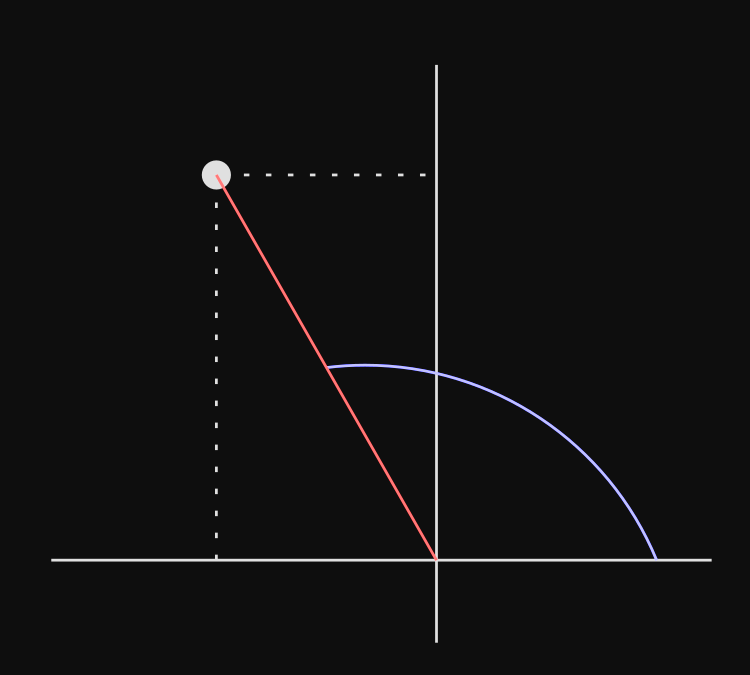
\includegraphics[scale=.125]{figures/polar-2.png}}
    {\tiny
    \put(2.20,0.04){$0$}
    \put(2.6,0.04){$x$}
    \put(2.05,0.9){$y$}
    \put(1.31,0.81){$(-2, 2\sqrt{3})$}}
    {\tiny
    \put(1.57,0.4){$2\sqrt{3}$}
    \put(1.89,0.05){$2$}}
    {\scriptsize
    \put(1.9,0.38){\alert{$4$}}
    \put(2.4,0.4){\textcolor{blue}{$\theta$}}
    }
    \end{picture}
\end{solution}
}
%-------------- end slide -------------------------------%}}}

%-------------- start slide -------------------------------%{{{ 27
\frame{
\begin{solution}[continued]
    The triangle sitting on the negative half of the real axis
    has sides of length $2$, $2\sqrt 3$, and $4$;
    \pause
    you should
    recognize this as a right triangle whose other two angles
    measure $\frac{\pi}{3}$ and $\frac{\pi}{6}$.
    \pause
    From this, we see that $\theta=\frac{2\pi}{3}$ is an
    argument of $z$.
    \pause

    \alert{Therefore, $z$ can be written in polar form as $z=4e^{i(2\pi/3)}.$}
    \pause
    \medskip

    The other approach to finding an argument, $\theta$,
    for $z=-2+2\sqrt{3}i$ is as follows.
    We've already calculated $|z|=r=4$.
    By definition, $\theta$ is an angle satisfying
    \pause
    \[ \cos\theta=\frac{-2}{4} \pause = -\frac{1}{2}
    \pause
    \quad\text{and}\quad
    \sin\theta=\frac{2\sqrt{3}}{4} \pause = \frac{\sqrt{3}}{2}.\]
    \pause
    By graphing the point $(-\frac{1}{2}, \frac{\sqrt{3}}{2})$,
    we again determine that $\theta=\frac{2\pi}{3}$, and thus
    \alert{$z$ can be written in polar form as $z=4e^{i(2\pi/3)}.$}
    \myQED
\end{solution}
}
%-------------- end slide -------------------------------%}}}

%-------------- start slide -------------------------------%{{{ 28
\frame{
\begin{problem}
    Convert each of the following complex numbers to polar form.
    \begin{enumerate}
        \item $3i$ \pause \textcolor{blue}{$=3e^{(\pi/2)i}$.} \pause
        \item $-1-i$ \pause \textcolor{blue}{$=\sqrt{2}e^{-(3\pi/4)i} \pause =\sqrt{2}e^{(5\pi/4)i}$.} \pause
        \item $\sqrt{3} - i$ \pause \textcolor{blue}{$=2e^{-(\pi/6)i}$.} \pause
        \item $\sqrt{3}+3i$ \pause \textcolor{blue}{=$2\sqrt{3}e^{(\pi/3)i}$.}
    \end{enumerate}
\end{problem}
}
%-------------- end slide -------------------------------%}}}

%-------------- start slide -------------------------------%{{{ 29
\frame{
\begin{problem}[ Converting from Polar Form to Cartesian form ]
    Let $z= 2e^{2\pi i / 3}$. Write $z$ in the form $z=a+bi$
    (this is called \alert{Cartesian form} or \alert{Standard form}).
\end{problem}
\vfill
\pause
\begin{solution}
    First, remember that $e^{i\theta}=\cos\theta +i\sin\theta$,
    \pause
    and thus
    \begin{eqnarray*}
        e^{2\pi i/3} & = & \cos (2 \pi /3) + i \sin(2\pi/3) \\ \pause
                     & = & -\frac{1}{2} + i \frac{\sqrt{3}}{2}.
    \end{eqnarray*}
    \pause
    Therefore
    \begin{eqnarray*}
    z = 2e^{2\pi i/3} \pause & = & 2 \left( -\frac{1}{2} + i \frac{\sqrt{3}}{3} \right) \\ \pause
                             & = & -1 + \sqrt{3} i.
    \end{eqnarray*}
\end{solution}
}
%-------------- end slide -------------------------------%}}}

%-------------- start slide -------------------------------%{{{ 30
\frame{
\begin{problem}
    Express each of the following complex numbers in Cartesian form.
    \begin{enumerate}
        \item $3e^{-\pi i}$
        \pause
        \textcolor{blue}{$=-3$}
        \pause
        \item $2e^{3\pi i/4}$
        \pause
        \textcolor{blue}{$=-\sqrt{2}+i\sqrt{2}$}
        \pause
        \item $2\sqrt{3}e^{-2\pi i/6}$
        \pause
        \textcolor{blue}{$=\sqrt{3}-3i$}
    \end{enumerate}
\end{problem}

}
%-------------- end slide -------------------------------%}}}

%-------------- start slide -------------------------------%{{{ 31
\frame{
\begin{emptytitle}
    Problems involving multiplication of complex numbers can often
    be solved more easily by using polar forms of the complex numbers.
\end{emptytitle}
\vfill
\pause
\begin{theorem}
    If $z_1=r_1e^{i\theta_1}$ and $z_2=r_2e^{i\theta_2}$
    are complex numbers, then
    \[ z_1z_2=r_1r_2e^{i(\theta_1+\theta_2)}\]
\end{theorem}
\pause
\vfill
\begin{theorem}[De Moivre's Theorem]
    If $\theta$ is any angle and $n$ is a positive integer,
    \[\left( e^{i \theta} \right)^n = e^{i n \theta}.\]
\end{theorem}
\pause
\vfill
\begin{emptytitle}
    As an immediate consequence of De Moivre's Theorem, we have that
    for any real number $r>0$ and any positive integer $n$,
    %%\[ \left( r\left( \cos \theta+i\sin \theta\right) \right)^{n}
    %%=r^{n}\left( \cos n \theta +i\sin n\theta\right). \]
    \begin{eqnarray*}
        (re^{i\theta})^n                                            & = & r^n e^{in\theta} \\
        \left( r\left( \cos \theta+i\sin \theta\right) \right) ^{n} & = & r^{n}\left( \cos n \theta +i\sin n\theta\right)
    \end{eqnarray*}
\end{emptytitle}
}
%-------------- end slide -------------------------------%}}}

%-------------- start slide -------------------------------%{{{ 32
\frame{
\begin{problem}
    Express $(1-i)^6(\sqrt{3}+i)^3$ in the form $a+bi$.
\end{problem}
\pause
\vfill
\begin{solution}
    Let $z=1-i=\sqrt{2}e^{-\pi i/4}$ and
    $w=\sqrt{3}+i=2e^{\pi i/6}$.
    \pause
    We want to compute $z^6w^3$.
    \pause
    \begin{eqnarray*}
        z^6w^3 & = & (\sqrt{2}e^{-\pi i/4})^6(2e^{\pi i/6})^3 \\ \pause
               & = & (2^3 e^{-6\pi i/4}) (2^3 e^{3\pi i/6})   \\ \pause
               & = & (8 e^{-3\pi i/2}) (8 e^{\pi i/2})        \\ \pause
               & = & 64 e^{-\pi i}                            \\ \pause
               & = & 64 e^{\pi i}                             \\ \pause
               & = & 64(\cos\pi + i\sin\pi)                   \\ \pause
               & = & -64.
    \end{eqnarray*}
\end{solution}
}
%-------------- end slide -------------------------------%}}}

%-------------- start slide -------------------------------%{{{ 33
\frame{
\begin{problem}
    Express $\left(\frac{1}{2}-\frac{\sqrt{3}}{2}i\right)^{17}$ in the form $a+bi$.
\end{problem}
\pause
\begin{solution}
    Let $z=\frac{1}{2}-\frac{\sqrt{3}}{2}i=e^{-\pi i/3}$.
    \pause
    Then
    \begin{eqnarray*}
        z^{17} & = & \left(e^{-\pi i/3}\right)^{17}        \\ \pause
               & = & e^{-17\pi i/3}                        \\ \pause
               & = & e^{\pi i/3}                           \\ \pause
               & = & \cos\frac{\pi}{3} +i\sin\frac{\pi}{3} \\ \pause
               & = & \frac{1}{2}+\frac{\sqrt{3}}{2}i.
    \end{eqnarray*}
\end{solution}
}
%-------------- end slide -------------------------------%}}}

\section[\textcolor{yellow}{}]{\textcolor{yellow}{Roots of Complex Numbers}}

%-------------- start slide -------------------------------%{{{ 34
\frame{
\frametitle{Roots of Complex Numbers}
\pause
\begin{definition}
    Let $z$ and $q$ be complex numbers, and let $n$ be a positive
    integer.
    \pause
    Then $z$ is called \alert{an $n^{th}$ root of $q$}
    if $z^n=q$.
\end{definition}
\pause
\vfill
\begin{alertblock}{De Moivre's Theorem and its implication}
    If $\theta$ is any angle and $n$ is a positive integer,
    $\left( e^{i \theta} \right)^n = e^{i n \theta}$.
    This implies that
    for any real number $r>0$ and any positive integer $n$,
    \[ (re^{i\theta})^n =r^ne^{i n\theta}. \]
    This leads to the following result.
\end{alertblock}
\pause
\vfill
\begin{corollary}
    Let $q$ be a nonzero complex number and $n$ a positive integer.
    Then $z^n=q$ has exactly $n$ complex solutions, i.e., $q$
    has exactly $n$ complex $n^{th}$ roots.
    %Let $z$ be a non zero complex number.
    %\index{complex numbers ! roots}Then there are always exactly $k$ many  $k^{th}$
    %roots of $z$ in $\mathbb{C}$.
\end{corollary}
}
%-------------- end slide -------------------------------%}}}

%-------------- start slide -------------------------------%{{{ 35
\frame{
\begin{example}
    For any positive real number $a$, $z^2=a$ has two complex
    (in this case, real) solution, $z=\sqrt{a}$ and $z=-\sqrt{a}$.
    This is equivalent to the statement that $a$ has two complex
    (in this case, real) square roots.
    \pause
    \begin{itemize}
        \item One particular example: $25$ has two square roots, $5$ and $-5$, and
            these are the two solutions to $z^2=25$.
            \pause
        \item But we all knew that. A more interesting example is that $-1$ has no
            real square roots, but suddenly it has two (complex) square roots, $i$
            and $-i$.  These are the two (complex) solutions to $z^2=1$.
    \end{itemize}
\end{example}
}
%-------------- end slide -------------------------------%}}}

%-------------- start slide -------------------------------%{{{ 36
\frame{
\begin{example}[ Cube Roots ]
    To find the (three) cube roots of $i$, we solve the equation
    $z^3=i$.
    \pause
    To do so, we express both $z$ and $i$ in polar form: convert
    $i$ to polar form, and write $z=re^{i\theta}$, giving us
    \vspace*{-.25in}

    \[ (re^{i\theta})^3 =\pause e^{\pi i/2}.\]
    \vspace*{-.2in}

    \pause
    Thus
    $r^3e^{3i\theta}=1e^{\pi i/2}$,
    \pause
    implying that
    $\textcolor{blue}{r^3=1}
    \pause
    \quad\text{and}\quad \alert{3\theta = \frac{\pi}{2}}$.
    \pause
    \begin{itemize}
        \item \textcolor{blue}{Since $r$ is a real number, $r^3=1$ implies
            that $r=1$.}
            \pause
        \item The statement $\alert{3\theta = \frac{\pi}{2}}$
            is \alert{not completely correct}.
            \pause
            The problem that arises is that the argument for $i$, $\frac{\pi}{2}$
            is not unique.
            \pause
            Instead, we could have written
            \vspace*{-.1in}

            \[ i=e^{5\pi i/2}\mbox{ or } i=e^{9\pi i/2}\mbox{ or } i=e^{-3\pi i/2}.\]
            \vspace*{-.2in}

            \pause
            \alert{In fact, there are infinitely many choices for the argument
            of $i$.}
            \pause
            The important thing to notice is that any two different arguments differ
            by a multiple of $2\pi$,
            \pause
            and thus we may write
            \vspace*{-.1in}

            \[ 3\theta = \frac{\pi}{2} + 2\pi\ell,~\ell\in\ZZ.\]
            \vspace*{-.2in}

            \pause
            ($\ZZ$ denotes the set of integers:
            $\{ \ldots, -3, -2, -1, 0,1, 2,3,\ldots\}$).
    \end{itemize}
\end{example}
}
%-----------------------end slide---------------------------%}}}

%-------------- start slide -------------------------------%{{{ 37
\frame{
\begin{example}[continued]
    Dividing both sides of $3\theta = \frac{\pi}{2} + 2\pi\ell$
    by $3$:
    \[ \theta = \frac{\pi}{6} + \frac{2}{3}\pi\ell,\]
    where $\ell$ is any integer.
    \pause
    The Corollary to De Moivre's Theorem tells us that there are only
    \alert{three} different cube roots.
    \pause
    These are obtained by using $\ell=0$, $\ell=1$, and $\ell=2$,
    resulting in three values of $\theta$:
    \pause
    \[ \frac{\pi}{6}, \frac{5\pi}{6},
    \quad\text{and}\quad \frac{9\pi}{6}=\frac{3\pi}{2}.\]
    \pause
    Thus the cube roots of $i$ are
    \[ e^{\pi i/6}, e^{5\pi i/6}, \quad\text{and}\quad e^{3\pi i/2}.\]
    \pause
    We now convert these to Cartesian form.
\end{example}
}
%-----------------------end slide---------------------------%}}}

%-------------- start slide -------------------------------%{{{ 38
\frame{
\begin{example}[continued]
    \begin{eqnarray*}
        e^{\pi i/6}  & = & \pause \frac{\sqrt{3}}{2} +\frac{1}{2}i,  \\ \pause
        e^{\pi i/6}  & = & \pause -\frac{\sqrt{3}}{2} +\frac{1}{2}i, \\ \pause
        e^{3\pi i/2} & = & \pause -i .
    \end{eqnarray*}
    \pause
    \textcolor{blue}{You can check your work by computing the cube of each of
    these.}
\end{example}
\vfill
\pause
\begin{emptytitle}
    This process is summarized in the following procedure.
\end{emptytitle}
}
%-----------------------end slide---------------------------%}}}

%-------------- start slide -------------------------------%{{{ 39
\frame{
\begin{alertblock}{Finding Roots of a Complex Number}
    Let $w$ be a complex number. We wish to find the $n^{th}$ roots of $w$, that is all $z$ such that $z^n = w$.

    There are $n$ distinct $n^{th}$ roots and they can be found as follows:.
    \pause
    \begin{enumerate}
        \item[1.] Express both $z$ and $w$ in polar form $z=re^{i\theta}, w=se^{i\phi}$. Then $z^n = w$ becomes:
            \[
            (re^{i\theta})^n = r^n e^{i n \theta} = se^{i\phi}
            \]
            We need to solve for $r$ and $\theta$.
            \pause
        \item[2.] Solve the following two equations:
            \begin{eqnarray*}
                r^n &=& s
            \end{eqnarray*}
            \begin{eqnarray}
                \label{rootseqns}
                e^{i n \theta} &=& e^{i \phi}
            \end{eqnarray}
    \end{enumerate}
\end{alertblock}
}
%-----------------------end slide---------------------------%}}}

%-------------- start slide -------------------------------%{{{ 40
\frame{
\begin{alertblock}{Continued}
    \begin{enumerate}
        \item[3.] The solutions to $r^n = s$ are given by $r = \sqrt[n]{s}$.  \pause
        \item[4.] The solutions to $e^{i n \theta} = e^{i \phi}$ are given by:
            \[
            n\theta = \phi + 2\pi \ell,  \; \mbox{for} \; \ell = 0,1,2, \cdots, n-1
            \]
            or
            \[
            \theta = \frac{\phi}{n} + \frac{2}{n} \pi \ell, \; \mbox{for} \; \ell = 0,1,2, \cdots, n-1
            \]
            \pause
        \item[5.]
            Using the solutions $r, \theta$ to the equations given in (\ref{rootseqns})
            construct the $n^{th}$ roots of the form $z = re^{i\theta}$.
    \end{enumerate}
\end{alertblock}
}
%-----------------------end slide---------------------------%}}}

%-------------- start slide -------------------------------%{{{ 41
\frame{
\begin{problem}
    Find all complex numbers $z$ such that
    $z^4=2(\sqrt{3}i-1)$,
    and express each in the form $a+bi$.
\end{problem}
\pause
\vfill
\begin{solution}
    \begin{enumerate}
        \item[1.] Convert $2(\sqrt{3}i-1)=-2+2\sqrt{3}i$ to polar form:
            \pause
            \[ |z^4|=\sqrt{(-2)^2+(2\sqrt{3})^2} =\sqrt{16}=4. \]

            \pause
            If $\phi$ is an argument for $-2+2\sqrt{3}i$, then
            \[\cos\phi = \frac{-2}{4}=-\frac{1}{2}
                \quad\text{and}\quad
                \sin\phi = \frac{2\sqrt{3}}{4}=\frac{\sqrt{3}}{2},
            \mbox{ so } \phi = \frac{2\pi}{3}.\]
            \pause
            Thus
            $z^4 = 4 e^{2\pi i/3}$.
            \pause
            Let $z=re^{i\theta}$.
            \pause
        \item[2.]
            The equation becomes $r^4e^{i4\theta} =  4 e^{2\pi i/3}$, so we need to solve
            \begin{eqnarray*}
                r^4&=&4 \\
                e^{i4\theta} &=& e^{2\pi i/3}
            \end{eqnarray*}
    \end{enumerate}
\end{solution}
}
%-----------------------end slide---------------------------%}}}

%-------------- start slide -------------------------------%{{{ 42
\frame{
\begin{solution}[continued]
    \begin{enumerate}
        \item[3.] Since $r^4=4$, $r^2=\pm 2$.  But $r$ is \alert{real}, and so
            $r^2=2$, implying $r=\pm\sqrt{2}$.
            However $r\geq 0$, and therefore $r=\sqrt{2}$.
            \pause
        \item[4.] The solutions to $e^{i4\theta} = e^{2\pi i/3}$ are given by
            \[ 4\theta = \frac{2}{3}\pi +2\pi \ell, \ell=0, 1, 2, 3.\]
            \pause
            Therefore,
            \[ \theta =  \frac{2\pi}{12} + \frac{2\pi \ell}{4}
             =  \frac{\pi}{6} + \frac{\pi \ell}{2}
             =  \frac{\pi(3\ell+1)}{6},
            \mbox{ for } \ell =0,1,2,3.\]
    \end{enumerate}
\end{solution}
}
%-----------------------end slide---------------------------%}}}

%-------------- start slide -------------------------------%{{{ 43
\frame{
\begin{solution}[continued]
    \begin{enumerate}
        \item[5.] Thus $r=\sqrt{2}$ and
            $\theta= \left(\frac{3\ell +1}{6}\right)\pi$, $\ell =0,1,2,3$.
            \pause
            Converting to Cartesian form:
            \pause
            \[ \begin{array}{llll}
            \ell =0: & z=\sqrt{2}e^{\pi i/6} & =
            \sqrt{2}(\frac{(\sqrt{3}}{2} + \frac{1}{2}i) &
            =\frac{\sqrt{6}}{2} + \frac{\sqrt{2}}{2}i \\
            \pause
            \ell =1: & z=\sqrt{2}e^{2\pi i/3} & =
            \sqrt{2}(-\frac{1}{2} + \frac{\sqrt{3}}{2}i)  &
            = -\frac{\sqrt{2}}{2} + \frac{\sqrt{6}}{2}i\\
            \pause
            \ell =2: & z=\sqrt{2}e^{7\pi i/6} & =
            \sqrt{2}(-\frac{\sqrt{3}}{2} - \frac{1}{2}i)  &
            =-\frac{\sqrt{6}}{2} - \frac{\sqrt{2}}{2}i \\
            \pause
            \ell =3: & z=\sqrt{2}e^{5\pi i/3} & =
            \sqrt{2}(\frac{1}{2} - \frac{\sqrt{3}}{2}i)  &
            = \frac{\sqrt{2}}{2} - \frac{\sqrt{6}}{2}i\\
            \end{array}\]
            \pause

            Therefore, the fourth roots of $2(\sqrt{3}i-1)$ are:
            \[ \frac{\sqrt{6}}{2} + \frac{\sqrt{2}}{2}i,
            \pause
            \textcolor{blue}{-\frac{\sqrt{2}}{2} + \frac{\sqrt{6}}{2}i},
            \pause
            -\frac{\sqrt{6}}{2} - \frac{\sqrt{2}}{2}i,
            \pause
            \textcolor{blue}{\frac{\sqrt{2}}{2} - \frac{\sqrt{6}}{2}i}.\]
            \myQED
    \end{enumerate}
\end{solution}
}
%-------------- end slide -------------------------------%}}}

\section[\textcolor{yellow}{}]{\textcolor{yellow}{Roots of Unity}}

%-------------- start slide -------------------------------%{{{ 44
\frame{
\frametitle{Roots of Unity}
\pause
\begin{definition}
    A complex number $z$ is a \alert{root of unity} if there
    exists a positive integer $n$ so that $z^n=1$.
\end{definition}
\pause
\vfill
\begin{problem}
    Find the sixth roots of unity, i.e., all solutions to $z^6=1$.
\end{problem}
\pause
\vfill
\begin{solution}
    Write $z=re^{i\theta}$ and convert $1$ to polar form to get
    \[ (re^{i\theta})^6 = e^{i0},\mbox{ and so } r^6e^{6\theta i} = e^{i0}.\]
    \pause
    Equating the absolute values and arguments,
    \[ r^6=1 \quad\text{and}\quad 6\theta = 0 + 2\pi \ell,~\ell=0,1,2,3,4,5.\]
    \pause
    Since $r$ is real, $r=1$.
    \pause
    The six arguments for the solutions are
    \[ \theta=\frac{2\pi\ell}{6}=\frac{\pi\ell}{3},~\ell = 0,1,2,3,4,5.\]
\end{solution}
}
%-------------- end slide -------------------------------%}}}

%-------------- start slide -------------------------------%{{{ 45
\frame{
\begin{solution}[continued]
    The six arguments for the solutions are
    \[ \theta=\frac{2\pi\ell}{6}=\frac{\pi\ell}{3},~\ell = 0,1,2,3,4,5.\]
    \pause
    Converting these to Cartesian form:
    \pause
    \[ \begin{array}{l|l|l}
        \ell & \theta & z \\ \hline \hline
        % & & \\
        0 & 0 & e^{0i}=1 \\
        \pause
        \textcolor{blue}{1} & \textcolor{blue}{\frac{\pi}{3}} &
        \textcolor{blue}{e^{\pi i/3}=\frac{1}{2} + \frac{\sqrt{3}}{2}i} \\
        \pause
        2 & \frac{2\pi}{3} & e^{2\pi i/3}=-\frac{1}{2} + \frac{\sqrt{3}}{2}i \\
        \pause
        \textcolor{blue}{3} & \textcolor{blue}{\pi} &
        \textcolor{blue}{e^{\pi i}=-1} \\
        \pause
        4 & \frac{4\pi}{3} & e^{4\pi i/3}=-\frac{1}{2} - \frac{\sqrt{3}}{2}i \\
        \pause
        \textcolor{blue}{5} & \textcolor{blue}{\frac{5\pi}{3}} &
        \textcolor{blue}{e^{5\pi i/3}=\frac{1}{2} - \frac{\sqrt{3}}{2}i}
    \end{array}\]
    \pause
    If you graph these six point in the complex plane, you'll see
    that they result in six equally spaced points on the unit circle,
    one of them being $(1,0)$.
    \myQED
\end{solution}
}
%-------------- end slide -------------------------------%}}}

%-------------- start slide -------------------------------%{{{ 46
\frame{
\begin{definition}{Roots of Unity}
    For any integer $n\geq 1$, the (complex) solutions to $z^n=1$ are
    \[ z=e^{2\pi\ell i / n} \mbox{ for } \ell=0,1,2,\ldots,n-1.\]
    \pause
    Furthermore, the $n^{th}$ roots of unity correspond to $n$
    equally spaced points on the unit circle, one of them being
    $(1,0)$.
\end{definition}
}
%-------------- end slide -------------------------------%}}}

\section[\textcolor{yellow}{}]{\textcolor{yellow}{The Quadratic Formula}}

%-------------- start slide -------------------------------%{{{ 47
\frame{
\frametitle{The Quadratic Formula}
\pause
\begin{definition}
    A \alert{real} quadratic is an expression of the form
    $ax^2+bx+c$ where $a, b, c\in\RR$ and $a\neq 0$.
\end{definition}
\vfill
\pause
\begin{emptytitle}
    To find the roots of a real quadratic, we can either
    factor by inspection, or use the \alert{quadratic formula}:
    \[ x= \frac{-b \pm\sqrt{b^2-4ac}}{2a} \]
    \pause
    The expression $b^2-4ac$ is called the \alert{discriminant}, \pause and
    \begin{itemize}
        \item if $b^2-4ac\geq 0$, then the roots of the quadratic are \alert{real}; \pause
        \item if $b^2-4ac<0$, then the quadratic has \alert{no real roots}.
    \end{itemize}
\end{emptytitle}
}
%-------------- end slide -------------------------------%}}}

%-------------- start slide -------------------------------%{{{ 48
\frame{
\begin{definition}
    A real quadratic $ax^2+bx+c$ is called
    \alert{irreducible} if the discriminant is less than zero,
    i.e., $b^2-4ac<0$.
\end{definition}
\pause
\begin{emptytitle}
    Notice that if $b^2-4ac<0$, then
    \[
    \sqrt{b^2-4ac}=\sqrt{(-1)(4ac-b^2)} = (\pm) i\sqrt{4ac-b^2}.\]
    \pause
    It follows that the roots of an irreducible quadratic are
    \[ \frac{-b\pm i\sqrt{4ac-b^2}}{2a}
    =\left\{ \begin{array}{l}\vspace*{.02in}
    -\frac{b}{2a} + \frac{\sqrt{4ac-b^2}}{2a}i \\
    -\frac{b}{2a} - \frac{\sqrt{4ac-b^2}}{2a}i
    \end{array}\right. ,
    \]
    \pause
    and we see that
    the two roots are complex conjugates of each other.
    \pause

    We denote the two roots by
    \[ u = -\frac{b}{2a} + \frac{\sqrt{4ac-b^2}}{2a}i
    \quad\text{and}\quad
    \overline{u}= -\frac{b}{2a} - \frac{\sqrt{4ac-b^2}}{2a}i. \]
\end{emptytitle}
}
%-------------- end slide -------------------------------%}}}

%-------------- start slide -------------------------------%{{{ 49
\frame{
\begin{example}[ Real Quadratics with Complex Roots ]
    The quadratic $x^2-14x+58$ has roots
    \begin{eqnarray*}
        x & = & \frac{14 \pm\sqrt{196-4\times 58}}{2} \\ \pause
          & = & \frac{14 \pm\sqrt{196-232}}{2}        \\ \pause
          & = & \frac{14 \pm\sqrt{-36}}{2}            \\ \pause
          & = & \frac{14 \pm 6i}{2}                   \\ \pause
          & = & 7\pm 3i,
    \end{eqnarray*}
    \pause
    so the roots are $7+3i$ and $7-3i$.
\end{example}
}
%-------------- end slide -------------------------------%}}}

%-------------- start slide -------------------------------%{{{ 50
\frame{
\begin{emptytitle}
    Conversely, given $u=a+bi$ with $b\neq 0$, there is an
    irreducible quadratic having roots $u$ and $\overline{u}$.
\end{emptytitle}
\pause
\vfill
\begin{problem}
    Find an irreducible quadratic with $u=5-2i$ as a root.  What is the other root?
\end{problem}
\pause
\vfill
\begin{solution}
    \begin{eqnarray*}
    (x-u)(x-\overline{u}) & = & \pause (x-(5-2i))(x-(5+2i)) \\
    \pause
    & = & x^2 -(5-2i)x -(5+2i)x +(5-2i)(5+2i) \\
    \pause
    & = & x^2-10x+29.
    \end{eqnarray*}
    \pause
    Therefore, $x^2-10x+29$ is an irreducible quadratic with
    roots $5-2i$ and $5+2i$.
    \pause

    \alert{Notice that $-10 = -(u+\overline{u})$ and
    $29=u\overline{u}=|u|^2$.}
    \myQED
\end{solution}
}
%-------------- end slide -------------------------------%}}}

%-------------- start slide -------------------------------%{{{ 51
\frame{
\begin{problem}
    Find an irreducible quadratic with root $u=-3+4i$, and find the other root.
\end{problem}
\vfill
\pause
\begin{solution}[ answer ]
    $x^2+6x+25$ has roots $u=-3+4i$ and $\overline{u}=-3-4i$.
\end{solution}
}
%-------------- end slide -------------------------------%}}}

%-------------- start slide -------------------------------%{{{ 52
\frame{
\begin{problem}[ Quadratics with Complex Coefficients ]
    Find the roots of the quadratic $x^2-(3-2i)x+(5-i)=0$.
\end{problem}
\pause
\vfill
\begin{solution}
    Using the quadratic formula
    \[ x=\frac{3-2i \pm\sqrt{ (-(3-2i))^2-4(5-i)}}{2}. \]
    \pause
    Now,
    \[  (-(3-2i))^2-4(5-i) = 5-12i-20+4i=-15-8i,\]
    \pause
    so
    \[ x=\frac{3-2i \pm\sqrt{-15-8i}}{2}. \]
    \pause
    To find $\pm\sqrt{-15-8i}$, solve $z^2=-15-8i$ for $z$.
\end{solution}
}
%-------------- end slide -------------------------------%}}}

%-------------- start slide -------------------------------%{{{ 53
\frame{
\begin{solution}[continued]
    Let $z=a+bi$ and $z^2=-15-8i$.
    \pause
    Then
    \[ (a^2-b^2)+2abi=-15-8i,\]
    \pause
    so $a^2-b^2=-15$ and $2ab=-8$.
    \medskip

    \pause
    Solving for $a$ and $b$ gives us
    $z= 1-4i, -1+4i$, i.e., $z=\pm(1-4i)$.
    \pause

    Therefore,
    \[ x=\frac{3-2i \pm(1-4i)}{2}, \]
    \pause
    and
    \[\begin{array}{l}
        \frac{3-2i +(1-4i)}{2} = \frac{4-6i}{2} = 2-3i,\\ \\
        \frac{3-2i -(1-4i)}{2} = \frac{2+2i}{2} = 1+i.
    \end{array}\]
    \pause
    Thus the roots of $x^2-(3-2i)x+(5-i)$ are $2-3i$ and $1+i$.
    \myQED
\end{solution}
}
%-------------- end slide -------------------------------%}}}

%-------------- start slide -------------------------------%{{{ 54
\frame{
\begin{problem}
    Find the roots of $x^2-3ix+(-3+i)$.
\end{problem}
\vfill
\pause
\begin{solution}[ answer ]
    $1+i$ and $-1+2i$.
\end{solution}
}
%-------------- end slide -------------------------------%}}}

%-------------- start slide -------------------------------%{{{ 55
\frame{
\begin{problem}
    Verify that $u_1=(4-i)$ is a root of
    \[ x^2-(2-3i)x-(10+6i) \]
    and find the other root, $u_2$.
\end{problem}
\pause
\vfill
\begin{solution}
    First,
    \begin{eqnarray*}
    u_1^2 -(2-3i)u_1 -(10+6i) & = & (4-i)^2-(2-3i)(4-i)-(10+6i) \\
                              & = & (15-8i)-(5-14i)-(10+6i)     \\
                              & = & 0,
    \end{eqnarray*}
    so $u_1=(4-i)$ is a root.
\end{solution}
}
%-------------- end slide -------------------------------%}}}

%-------------- start slide -------------------------------%{{{ 56
\frame{
\begin{solution}[continued]
    Recall that if $u_1$ and $u_2$ are the roots of the quadratic,
    then
    \[ u_1 + u_2 = (2-3i) \quad\text{and}\quad u_1u_2 = -(10+6i). \]
    Solve for $u_2$ using either one of these equations.
    \pause

    Since $u_1=4-i$ and $u_1+u_2=2-3i$,
    \[ u_2=2-3i-u_1=2-3i-(4-i)=-2-2i.\]
    \pause
    Therefore, the other root is $u_2=-2-2i$.
    \pause

    You can easily verify your answer by computing $u_1u_2$:
    \[ u_1u_2=(4-i)(-2-2i)= -10 -6i=-(10+6i).\]
    \myQED
\end{solution}
}
%-------------- end slide -------------------------------%}}}

\end{document}
